\documentclass[12pt, a4paper, oneside]{ctexbook}
\usepackage{amsmath, amsthm, amssymb, bm, graphicx, hyperref, mathrsfs}

\title{{\Huge{\textbf{现代数学前沿概览}}}\\——副标题}
\author{Dylaaan}
\date{\today}
\linespread{1.5}
\newtheorem{theorem}{定理}[section]
\newtheorem{definition}[theorem]{定义}
\newtheorem{lemma}[theorem]{引理}
\newtheorem{corollary}[theorem]{推论}
\newtheorem{example}[theorem]{例}
\newtheorem{proposition}[theorem]{命题}

\begin{document}

\maketitle

\pagenumbering{roman}
\setcounter{page}{1}

\begin{center}
    \Huge\textbf{前言}
\end{center}~\

这是笔记的前言部分.
~\\
\begin{flushright}
    \begin{tabular}{c}
        Dylaaan \\
        \today
    \end{tabular}
\end{flushright}

\newpage
\pagenumbering{Roman}
\setcounter{page}{1}
\tableofcontents
\newpage
\setcounter{page}{1}
\pagenumbering{arabic}

\chapter{思考题}
\subsection*{1. 简述霍尔效应现象及其物理原理。}
当电流垂直于外磁场通过导体时,载流子发生偏转,在垂直于电流和磁场的方向会产
生一附加电场,从而在导体的两端产生电势差$ U $ ,$ U $ 被称为电势差。
\subsection*{ 在霍尔效应测量中,霍尔电压的正负号是如何约定的?
    如右图所示,根据约定,测量霍尔电压时,电压表的正极应该接在 A
    点还是 B 点?}
霍尔电压的正负由载流子受到的洛伦兹力影响,具体来说沿$ B\times v $的方向为从负到正; 如果载流子是正电荷(空穴),那么应当A接正极,B接负极。反之如果载流子是电子,那么A,B的极性相反,A接负极,B接正极。
\subsection*{对于磁电阻元件样品(参看讲义图 4),若 C、D 端通入恒定工作电流 I,垂直样品表面方向
    施加如下图所示的较弱的交流磁场 B,请画出在样品工作电流方向上的电压降 UCD 的示意图
    (实验中可以进行研究性验证)}
在磁场较弱时,一般正常磁阻器件的$ \Delta R(0) $ 正比于$ B^2 $,也即$$
    \frac{\Delta R}{R}=kB^2
$$
故$$
    U_{CD}=R(B)\cdot I=(1+kB^2)R(0)\cdot I
$$
\newpage
\subsection*{示波器的使用}
包括使用trigger按钮调整触发电平使波形稳定、用meas按钮进行波形的测量,以及cursor按钮调整指针。

除此之外,autoscale可以帮助我们自动调整波形,水平调节旋钮可以调节时间轴,horizontal键可以调节时基长度等等

值得注意的是,示波器的探头$ \times 1 $ 和$ \times 10 $ 档的区别,在测量高频和低频信号时要注意区别

一般来说,示波器的使用基本上就是上面所说的一些功能。
\subsection*{查阅资料,列举超声波在日常工业及医疗等方面 2~3 个具体应用。}
1.超声波用于焊接:超声波用于焊接塑料,高频超声波振动将塑料的几个零部件焊接在一起。

2.超声波运动探测器在测量距离时使用相同的超声波。

3.超声波用于清洗,它用于去除某些被水溶液吸收的装置中的杂质

\subsection*{ 利用超声斜探头探测试样中缺陷 D 的位置的方法,设计方案,写出测量公式}
用直探头可以探测出D孔的深度,但不能测得其水平距离,因此采用斜探头确定D孔在试块中的横向位置。D孔的深度为$ H_D $ ,水平距离为
$$
    X=L+X_{\mathrm{00}}-L^{'}
$$
$ \beta $ 是斜探头在被测试块中的折射角,只要知道 $L_{D},X_{00},L^{'}$ ,$ \beta $的值就可计算出$ H_D $

$X_D$的值。
\begin{figure}[!h]
    \begin{center}
        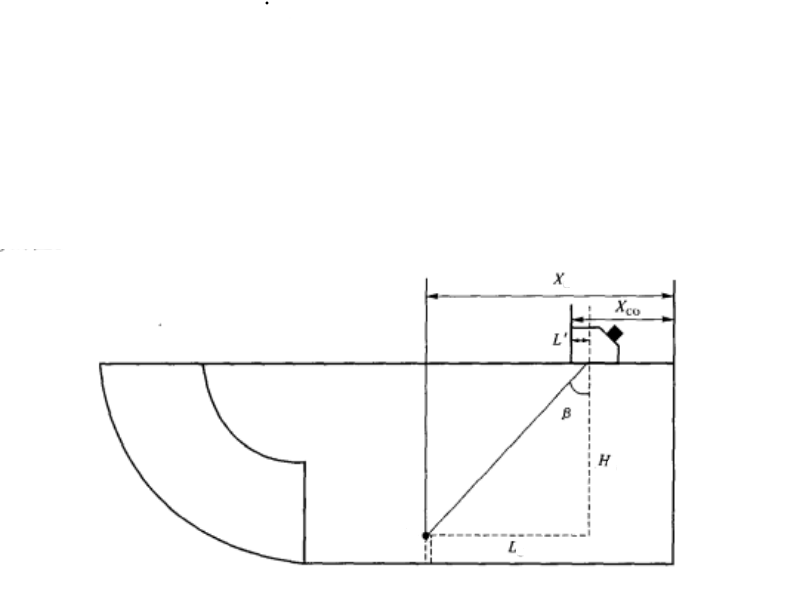
\includegraphics[scale=0.8]{XA.png}
    \end{center}
\end{figure}

第一步:测探头的前沿与入射点的距离 $L$ ,观察R,和R,的反射回

波,前后移动探头,使R, 与Rz面的反射回波最大,用米尺测量探头前沿到工件端点的距离L,进而得到探头的前沿与人射点的距离 $L$ :

$$
    L^{'}=R_{2}-L
$$
第二步:利用R,和 Rz反射面测量斜探头的延迟时间 t。和声速v,
$$
    t_0=2t_1-t_2
$$
$$
    v=\frac{2(R_{2}-R_{1})}{t_{2}-t_{1}}
$$
第三步:用试块中已知位置的横通孔A和B测量斜探头的折射角β
$$
    \quad tg\beta=\frac{S}{H_{AB}}
$$
其中,A,B为试块中的两个已知位置的横孔,让斜探头先后找到孔A和B的最大反射回波,分别测量出探头前沿到端面的水平距离为$ L_A、L_B $ ,已知它们的深度为$ H_A、H_B $ ,则有
$$
    S=L_{B O}-L_{A O}-L_{A B}
$$
$$
    H_{A B}=H_{B}-H_{A B}
$$
\begin{figure}[!h]
    \begin{center}
        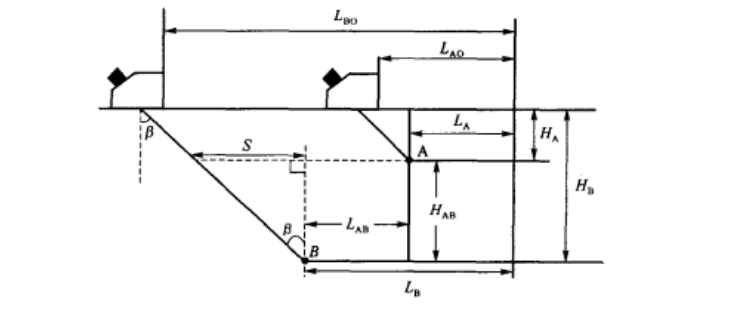
\includegraphics{X.png}
    \end{center}
\end{figure}
折射角:
$$
    \beta=\mathfrak{t g}^{-1}\left(\frac{S}{H_{\mathrm{AB}}}\right)
$$
第四步:用斜探头找出D孔的最大反射回波的位置,用示波器读出$ t_c $ ,根据已测出的
$ v $ ,即可计算出 $H_{\mathrm{c}},X_{\mathrm{co}}$
\newpage
\subsection*{1. 简单说明逸出功的定义。}
是指电子从金属表面逸出时克服表面势垒必须做的功
\subsection*{阅读讲义并简述利用热电子发射法测金属钨电子逸出功的方法的巧妙之处。}
热电子发射是用提高阴极温度的办法以改变电子的能量分布,使动能大于 Wi 的电子增多,
从而使动能大于 Wa 的电子数达到一可观测的大小,
\subsection*{3. 请根据讲义内容尝试设计实验线路图(示意图)}
为了测量逸出功,我们依据式(2)测出参量 $ I_e,A,S  $ 及 T,利用式(2)就
可以求出金属的逸出功$  e_0\phi $.

首先由里查孙直线法测量$ A-S $

再直接测量$ I_e $,由表达式$$
    \lg I^{\prime}_{e}=\lg I_{e}+\frac{4.39}{2.303 T} \frac{1}{\sqrt{r_{1} \ln \left(r_{2} / r_{1}\right)}} \sqrt{U_{a}}
$$
我们外推$ U_a=0 $ 处即可求得$ I_e $

最后测$ T $ 。实验中测得钨丝加热电流 $ I_f $  后由前人测量的结果可通过线性插值法求出温度 T

总的来说,困难的地方在于如何消除副效应,并且绕开难以测量的$ A-S $ 关系。

\newpage
\subsection*{简单说明超导材料的两个基本性质:零电阻和完全抗磁性(迈斯纳效应)}
零电阻特性,超导体的电阻率在温度低于某一临界温度时迅速降至零、不存在可观测的直流电阻的特性。\\
完全抗磁性: 即超导体处于超导态时其内部磁感应强度为零$ \vec{B} = 0 $ ,与其先处于外磁场中再降温至超导态还是先进入超导态再施加外磁场的过程无关。
\subsection*{ 阅读讲义、查阅文献,了解超导材料发展的历史和现状。举一个超导材料可以应用的例子}
磁浮列车:超导材料可以制造高速磁浮列车中所需的强电磁场,使列车悬浮在轨道上,减少摩擦力和空气阻力,提高列车速度。

\subsection*{画出四极法(四端法)测电阻的示意图,四极法比两极法测电阻有什么优点?}
\begin{figure}[!h]
    \centering
    \caption{四极法测电阻示意图}
    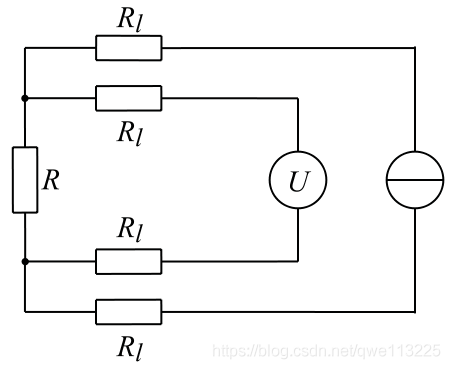
\includegraphics[scale=0.5]{sixianfa.png}
\end{figure}
相较于两极法,四极法测小电阻时更加精确。

4. 初级线圈和次级线圈平行排列,互感为 M0,
如右图所示。设初级线圈中通有电流$  i=i_0cos\omega t $

(1)次级线圈两端的感应电动势的有效值 $ U_{AB0} $
为$ -M_0i_0\omega /\sqrt{2} $
频率越高,$ U_{AB} $  \textbf{越大} \\

(2)如果两线圈之间插有一块样品。如下图所示
如果样品是顺磁性的,则次级线圈两端的感应电动势的有效值$ U_{AB} $ 比 $ U_{AB0} $ 大还是小?\\\textbf{大}\\
如果样品是抗磁性的,则次级线圈两端的感应电动势的有效值$ U_{AB} $ 比 $ U_{AB0} $ 大还是小?\\\textbf{小}\\
\newpage
\subsection*{查阅资料,学习(复习)分光计的结构原理及调节方法过程}
\begin{figure}
    \centering
    \caption{分光计的结构}
    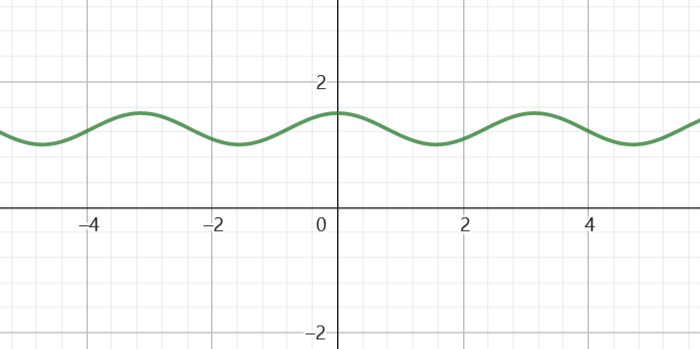
\includegraphics[scale=0.7]{a.png}
\end{figure}
\begin{itemize}
    \item[1] 调节望远镜适合于观察平行光
    \item[2] 调节望远镜光轴垂直于分光计主轴
    \item[3] 调节平行光管使产生平行光
    \item[4] 调节平行光管光轴垂直于分光计主轴
    \item[5] 调节三棱镜两个光学面的法线垂直于分光计主轴
\end{itemize}
分光计的调整应满足:望远镜适合于观察平行光,平行光管发出平行光,并且二者的光轴都垂直于分
光计主轴。
\subsection*{用公式(2)测 $ d $或$ \lambda $ 时,实验需要保证什么条件?}
在光线正入射即 i=0 的情况下测量时,公式(2)才成立。

\subsection*{什么是视差?如何判断存在视差?分光计调节过程中哪些环节需要消除视差?如何消除?}
视差就是从有一定距离的两个点上观察同一个目标所产生的方向差异;
改变观察方向,若原本观察的物体发生相对移动,则存在视差;调节望远镜和平行光管焦距时需要消除视差;调节镜筒至成像清晰,且移动视线不会引起像与叉丝发生相对位移。
\subsection*{由式(2)推导出$ d $和$ \lambda $ 的不确定度估算公式。为了减少测量误差,应根据观察到的各级谱线
    的强弱及不确定度的公式来决定测量第几级的$ \varphi_m $ 较为合理}

由公式(2)
$$
    dsin\varphi_m=m\lambda
$$
知$$
    \frac{\partial lnd}{\partial m}=\frac{1}{m},\quad \frac{\partial lnd}{\partial \lambda}=\frac{1}{\lambda},\quad \frac{\partial lnd}{\partial \varphi_m}=-\frac{1}{tan\varphi_m}
$$
则$d$的不确定度为$$
    \Delta d=d\sqrt{(\frac{\Delta m}{m})^{2}+(\frac{\Delta\lambda}{\lambda})^{2}+(\frac{\Delta\varphi_{m}}{tan\varphi_{m}})^{2}}
$$
又$ \Delta_m=\Delta_\lambda=0 $
则$$
    \Delta d=d\left|\frac{\Delta_{\varphi_m}}{tan\varphi_m}\right|
$$
$ \lambda $ 的不确定度同理,有$$
    \frac{\partial ln\lambda}{\partial m}=-\frac{1}{m},\quad \frac{\partial ln\lambda}{\partial d}=\frac{1}{d},\quad \frac{\partial ln\lambda}{\partial \varphi_m}=\frac{1}{tan\varphi_m}
$$
则$$
    \Delta\lambda=\lambda\sqrt{(\frac{\Delta d}{d})^{2}+(\frac{1}{t g\varphi_{m}})^{2}{\Delta\varphi_{m}}^{2}+(\frac{\Delta m}{m})^{2}}
$$
又$ \Delta_m=0 $
则$$
    \Delta\lambda=\lambda\sqrt{(\frac{\Delta d}{d})^{2}+(\frac{1}{tan\varphi_{m}})^{2}\Delta{\varphi_{m}}^{2}}
$$
由上述推导可知$ \varphi_m=arcsin\frac{m\lambda}{d} $越大,$ \Delta_\lambda,\Delta_d $ 就越小,因此在可观测的范围内,m取值越大越好
\end{document}
